\documentclass{article}
\usepackage[utf8]{inputenc}

\usepackage{graphicx}

\title{My First Paper with Overleaf and GitHub}
\author{Jacob R. Bradley, Timothy I. Cannings and Aris Sionakidis}
\date{April 2021}

\begin{document}

\maketitle

\section{Introduction}
I want to learn about methods for doing classification, i.e. for taking training data 

\[ T_n = \{ (X,Y): \ X \in R^p, Y \in \{0,1\}, \]

and predicting outcomes $Y$ from unseen data $X$.

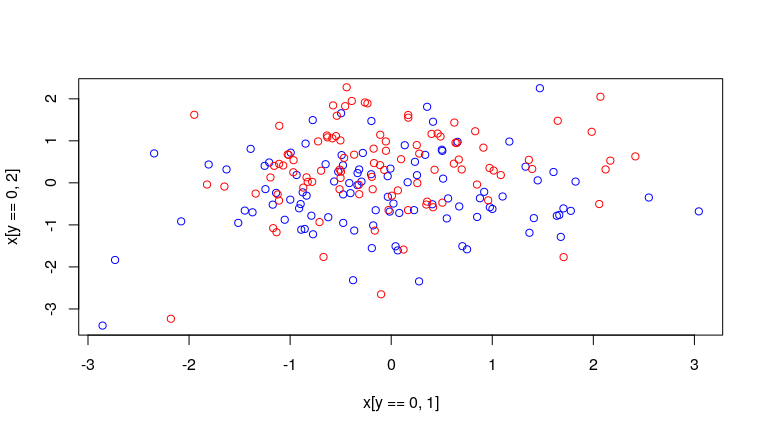
\includegraphics{results/figures/Rplot.png}

Look at this plot! Very revealing!

\subsection{Literature Review} 
People have worked on classification before - see for example \cite{cannings_random-projection_2017}.

\section{Section Two}

\bibliographystyle{plain}
\bibliography{references}

\end{document}
